\chapter{ Aufbau der optischen Diode}

Um eine destabilisierende Rückkopplung in den He-Ne-Resonator zu verhindern, setzen wir den Isolator ein, der im \cref{fig:function_of_optical_diode} dargestellt ist. 
Brewster-Fenster, so angebracht, dass sie im Brewster-Winkel \cite{introtoED} 
\begin{equation}
  \tan\theta_B = \bigl(\tfrac{n_{\mathrm{glas}}}{n_{\mathrm{luft}}}\bigr),
\end{equation}
stehen, dienen als erster Polarisationsfilter innerhalb der Kavität. 
Bei diesem Winkel passiert p-polarisiertes Licht (mit elektrischem Feld in der Einfallsebene) die Glas-Luft-Grenzfläche ohne Reflexion, während s-polarisiertes Licht (Feld senkrecht zur Einfallsebene) teilweise reflektiert und somit unterdrückt wird. 
Dadurch ist der intra-kavitär austretende Strahl am Ausgangskoppler bereits stark linear entlang der p-Achse polarisiert und liefert einen sauberen Eingangsstatus für die nachfolgenden Isolator-Komponenten.

\begin{figure}[htbp]
  \centering
  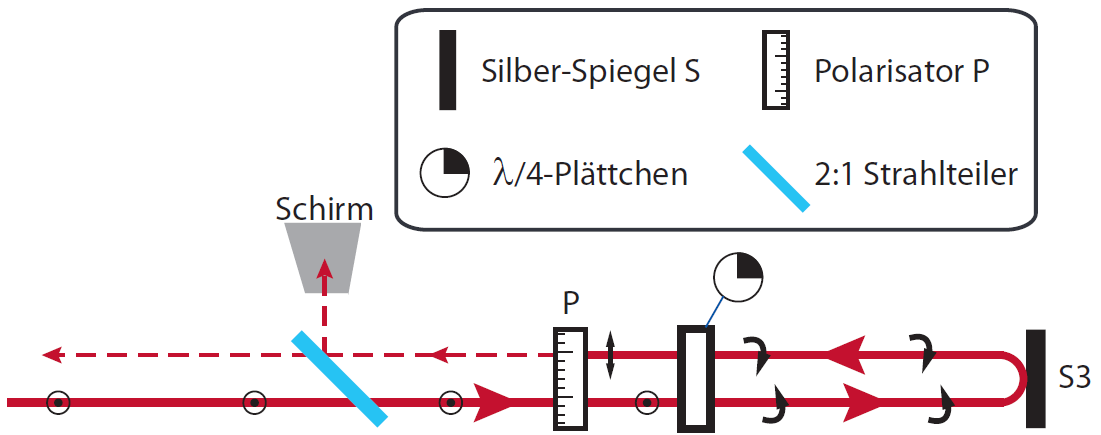
\includegraphics[width=0.75\linewidth]{Funktion der optischen Diode.png}
  \caption{Funktionsprinzip des optischen Isolators: Der rückwärts laufende Strahl ist zur Veranschaulichung leicht versetzt dargestellt. Schwarze Pfeile entlang des Strahlengangs zeigen mögliche Polarisationszustände in den einzelnen Stufen an.}
  \label{fig:function_of_optical_diode}
\end{figure}

Der Isolator selbst besteht aus einem linearen Polarisator (P), einer Viertelwellenplatte ($\lambda/4$) und einem Silber-Spiegel (S3), die unmittelbar hinter dem Ausgangskoppler in Serie angeordnet sind (siehe \cref{fig:aufbau_mit_optischer_diode}). 
Auf dem Vorwärtsdurchgang überträgt P nur das p-polarisierte Licht, welches die $\lambda/4$-Platte in rechtszirkulare Polarisation umwandelt. 
Nach der Reflexion an S3 - die Drehrichtung beibehält - durchläuft der Rückstrahl erneut die $\lambda/4$-Platte und tritt als um 90° gedrehtes, nun s-polarisiertes Licht aus. 
Dieses gedrehte Licht wird von P blockiert, sodass eine hohe nicht-reziproke Isolation erreicht wird, ohne nennenswerte Einfügedämpfung im Vorwärtsweg.
\begin{figure}[htbp]
  \centering
  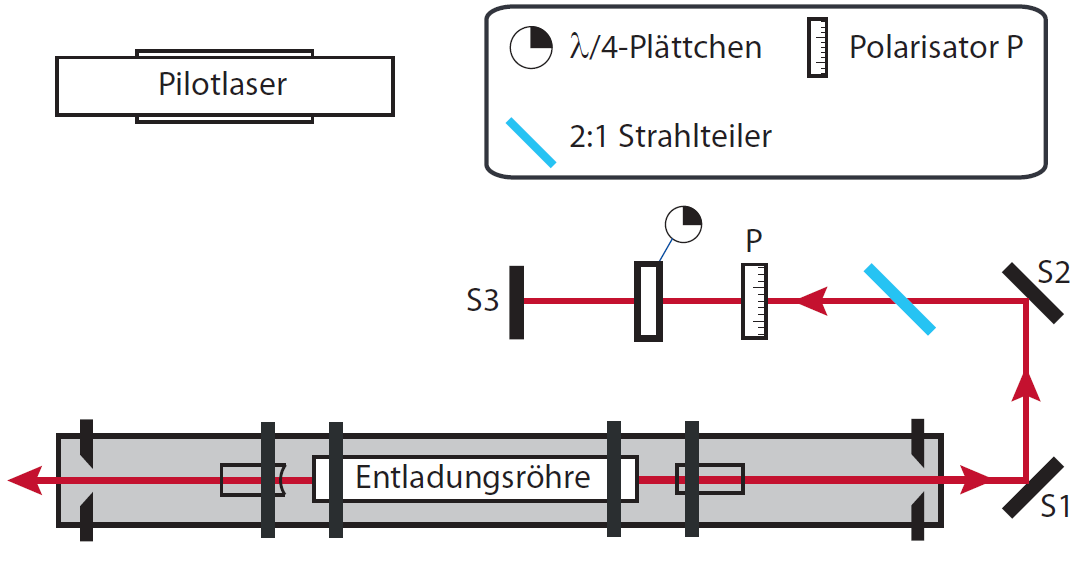
\includegraphics[width=0.75\linewidth]{Aufbau mit optischer Diode.png}
  \caption{Aufbau mit optischer Diode}
  \label{fig:aufbau_mit_optischer_diode}
\end{figure}

Mechanisch sind der Polarisator, die $\lambda/4$-Platte und ein nicht-polarisierender Strahlteiler im Verhältnis 2 : 1 in Justierhaltern montiert, die feines Kippen und Drehen sowie axiale Ausrichtung erlauben. 
Der Strahlteiler führt etwa ein Drittel des Vorwärtslichts zu einer Leistungsüberwachung ab, während der Rest zur schnellen Photodiodenkette gelangt. Alle Optiken verfügen über breitbandige Antireflexbeschichtungen, um Streureflexionen zu minimieren.

\paragraph{Justage-Prozedur:}
\begin{enumerate}
  \item \textbf{Polarisator-Orientierung:} Drehen Sie P, bis die durch den Monitorport gemessene Leistung maximal ist, um die native p-Polarisation des Lasers einzustellen.
  \item \textbf{Viertelwellenplatten-Einstellung:} Entfernen Sie S3 und justieren Sie die $\lambda/4$-Platte, bis die schwache Rückreflexion durch P auf einem Schirm verschwindet - ein Zeichen für eine perfekte 90°-Drehung der rücklaufenden Polarisation.
  \item \textbf{Isolations-Überprüfung:} Setzen Sie S3 wieder ein und vergewissern Sie sich, dass kein messbarer Rückfluss durch P auftritt, während die Vorwärtsdurchlässigkeit unverändert bleibt.  
\end{enumerate}
Während der Justage wurde der Polarisator auf $\theta = 290^\circ \pm 1^\circ$ und die Viertelwellenplatte auf $\lambda/4 = 64^\circ \pm 1^\circ$ eingestellt.


%===============================================================================================================================================================================================================================================================================================================================================
\chapter{Optischer Spektrumanalysator}

Nach Verlassen des Isolators wird der He-Ne-Strahl in einen konfokalen Fabry-Perot-Resonator (\cref{fig:Spektrumanalysator}) mit äußerer Länge $l_{\mathrm{ext}} = 5{,}0\,\si{\centi\meter}$ eingekoppelt. \\
Nach Handbuch \cite{praktikum} sind dessen Eigenfrequenzen
\begin{equation}
  \nu_{qnm}
  = \Bigl(q + \tfrac{m+n+1}{2}\Bigr)\,\frac{c}{2\,l}.
\end{equation}
Gleiche transversale Moden TEM$_{nm}$ liegen damit im Abstand des freien Spektralbereichs
\begin{equation*}
  \Delta\nu_{\mathrm{FSR}}
  = \frac{c}{2\,l},
\end{equation*}
während benachbarte Moden um
\begin{equation*}
  \Delta\nu
  = \frac{c}{4\,l}
\end{equation*}
getrennt sind.
\begin{figure}[htbp]
  \centering
  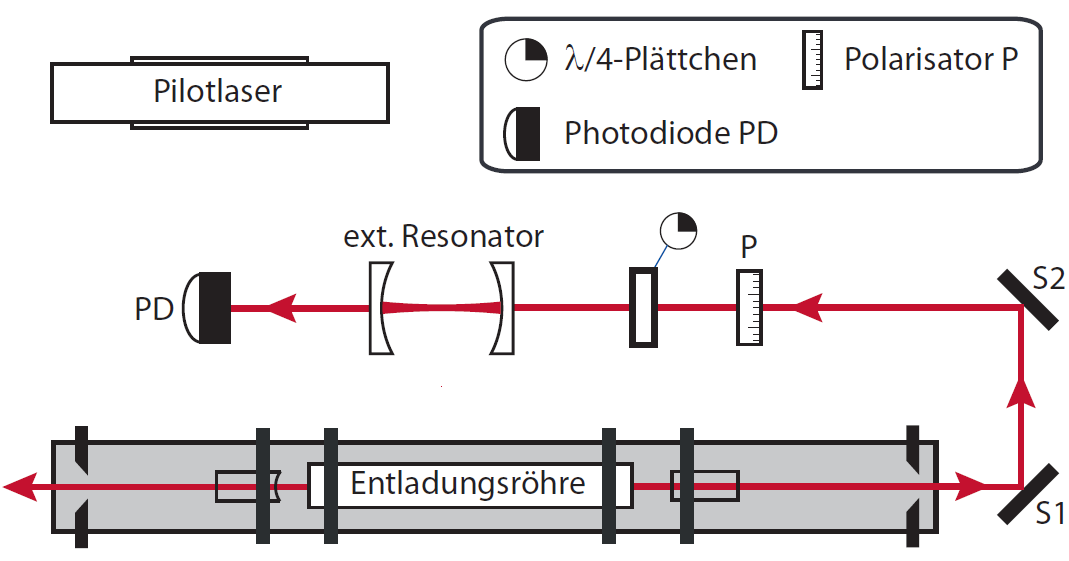
\includegraphics[width=0.75\linewidth]{Aufbaus zum optischen Spektrumanalysator.png}
  \caption{Schema des Aufbaus zum optischen Spektrumanalysator}
  \label{fig:Spektrumanalysator}
\end{figure}

Ein Piezoaktor verändert $l_{\mathrm{ext}} = 5 \si{\cm}$ um etwa $200\,\si{\nm}$ bei einer $0-100 \si{\volt}  $/$50 \si{\hertz}$-Dreiecksspannung, so dass ein vollständiger Sweep genau eine $\Delta\nu_{\mathrm{FSR}}$ abtastet. 
Kanal 1 des Oszilloskops zeigt die Piezo-Spannung $U(t)$, Kanal 2 die transmittierte Intensität $I(t)$ einer langsamen Photodiode, was eine Folge von Übertragungsclustern wie zwischen \cref{fig:9a} bis \cref{fig:9c} ergibt. 
Die korrekte Justage erfolgte mittels Papierziel- und Zwei-Spiegel-Kippverfahren (\cref{fig:Resonator}), bis für jede Piezo-Position ein einziger scharfer Spot auftrat und die Peaks minimal verbreitert waren.
\begin{figure}[htbp]
  \centering
  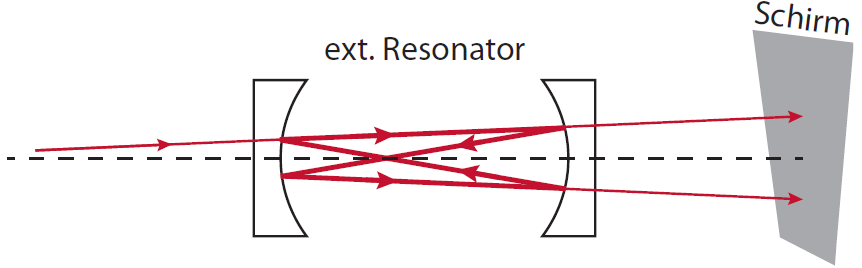
\includegraphics[width=0.75\linewidth]{Resonator bei Dejustage.png}
  \caption{Strahlengang im externen Resonator bei Dejustage}
  \label{fig:Resonator}
\end{figure}
\begin{figure}[htbp]
    \centering
    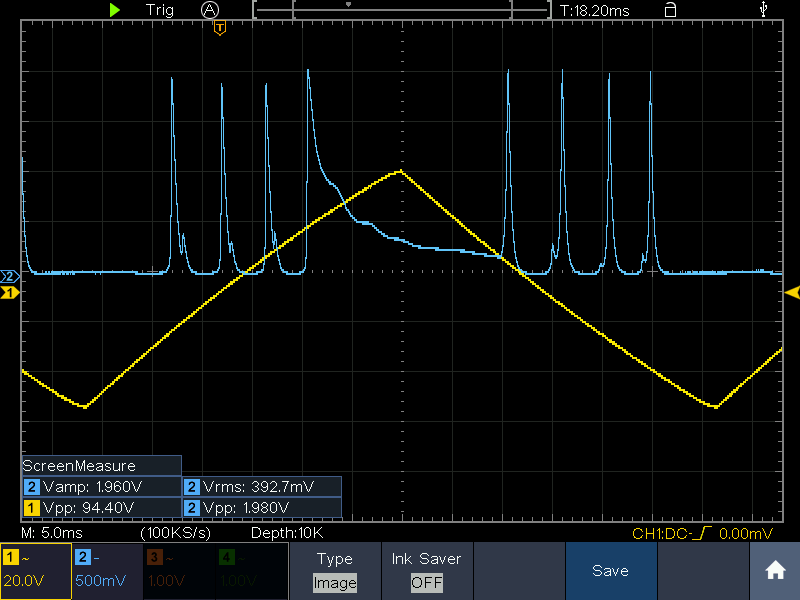
\includegraphics[width=0.75\linewidth]{52_1a.png}
     \caption{Oszilloskopübertragungscluster interne Kavitätenlängen $l = 52,0\,\si{\centi\meter} \pm$ 0{,}4\,\si{\centi\meter}.}
    \label{fig:9a}
\end{figure}
  \begin{figure}[htbp]
    \centering
    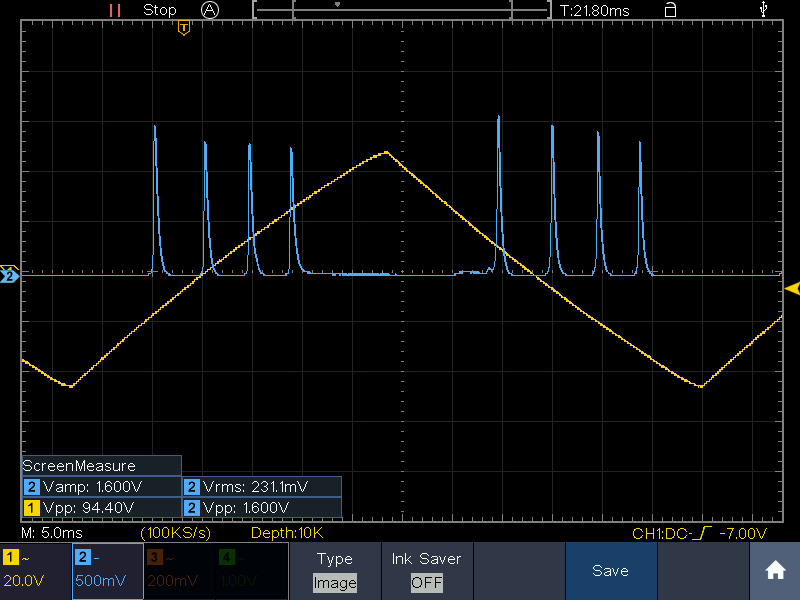
\includegraphics[width=0.75\linewidth]{68_1a.png}
     \caption{Oszilloskopübertragungscluste interne Kavitätenlängen $l = 68,0\,\si{\centi\meter} \pm$ 0{,}3\,\si{\centi\meter}.}
    \label{fig:9b}
  \end{figure}
  \newpage
  \begin{figure}[htbp]
    \centering
    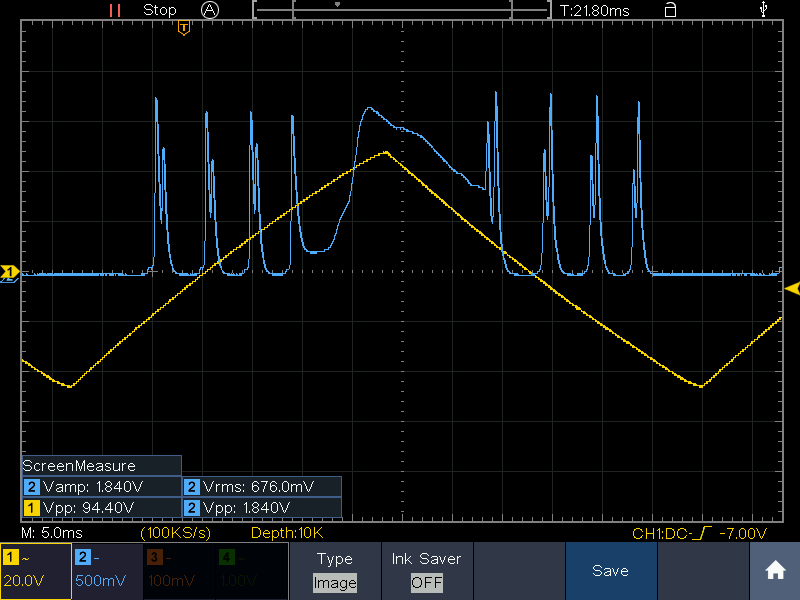
\includegraphics[width=0.75\linewidth]{80_1a.png}
     \caption{Oszilloskopübertragungscluster interne Kavitätenlängen $l = 80,0\,\si{\centi\meter} \pm$ 0{,}3\,\si{\centi\meter}.}
    \label{fig:9c}
  \end{figure}
 
 Für jede Oszilloskop-Spur bestimmen wir zwei Zeitintervalle: $a$, die horizontale Ausdehnung eines gesamten Übertragungsclusters (entspricht einer freien Spektralbreite des externen Fabry-Perot-Analysators), und $b$, der Abstand zweier benachbarter Peaks innerhalb dieses Clusters (entspricht dem longitudinalen Modenabstand der internen He-Ne-Kavität). 
 Da sowohl $a$ als auch $b$ auf derselben (möglicherweise nichtlinearen) Piezo-Zeitachse abgelesen werden, kompensiert ihr Verhältnis jede unbekannte Kalibrierkonstante. Damit lassen sich drei Frequenzintervalle definieren.

Die freie Spektralbreite des Analysators ist
\begin{equation}
  \Delta\nu_{\mathrm{FSR}}
  = \frac{c}{2\,l_{\mathrm{ext}}}
  = \frac{299\,792\,458\;\mathrm{m/s}}{2 \times 0{,}050\;\mathrm{m}}
  \approx 3{,}00\;\mathrm{GHz},
\end{equation}
wobei $l_{\mathrm{ext}} = 5{,}0\;\mathrm{cm}$.

Der experimentell bestimmte Modenabstand des Lasers ergibt sich zu
\begin{equation}
 \Delta\nu_{\mathrm{exp}}
  = \frac{b}{a}\;\Delta\nu_{\mathrm{FSR}},
\end{equation}
mit der Fehlerfortpflanzung
\begin{equation}
  \delta\Delta\nu_{\mathrm{exp}}
  =\Delta\nu_{\mathrm{exp}}
    \sqrt{\Bigl(\frac{\delta b}{b}\Bigr)^{2}
        + \Bigl(\frac{\delta a}{a}\Bigr)^{2}
        + \Bigl(\frac{\delta l}{l}\Bigr)^{2}}\!,
\end{equation}
wobei die Cursor-Unsicherheiten $\delta a = 0{,}20\;\mathrm{ms}$ und $\delta b = 0{,}20\;\mathrm{ms}$ sowie die Längenunsicherheiten $\delta l_{52} = 0{,}4\;\mathrm{cm}$ und $\delta l_{68} = \delta l_{80} = 0{,}3\;\mathrm{cm}$ betragen.

Der theoretische Modenabstand für eine ideale planparallele Kavität der Länge $l$ ist
\begin{equation}
 \Delta\nu_{\mathrm{theo}}
  = \frac{c}{2\,l},
  \quad
  \delta\Delta\nu_{\mathrm{theo}}
  =\Delta\nu_{\mathrm{theo}}\,\frac{\delta l}{l}.
\end{equation}

\begin{table}[H]
  \centering
  \resizebox{0.8\columnwidth}{!}{%
    \begin{tabular}{|c|c|c|c|c|}
      \hline
      $l \,\;\pm\delta l \,/\mathrm{cm}$ 
        & $a \,\pm \delta a\,/\mathrm{ms}$ 
        & $b \,\pm \delta b\,/\mathrm{ms}$ 
        & $v_{\mathrm{exp}}\pm\delta\Delta\nu_{\mathrm{exp}}\;/\;\mathrm{MHz}$ 
        & $v_{\mathrm{theo}}\pm\delta\Delta\nu_{\mathrm{theo}}\;/\;\mathrm{MHz}$ \\ \hline
      $52{,}0 \pm 0{,}4$   & $25{,}0 \pm 0{,}2$ & $3{,}0 \pm 0{,}2$ & $360 \pm 13$ & $288 \pm 2$ \\ \hline
      $68{,}0 \pm 0{,}3$   & $25{,}0 \pm 0{,}2$ & $2{,}0 \pm 0{,}2$ & $240 \pm 12$ & $220 \pm 1$ \\ \hline
      $80{,}0 \pm 0{,}3$   & $25{,}0\pm 0{,}2$ & $1{,}5 \pm 0{,}2$ & $180 \pm 12$ & $187 \pm 1$ \\ \hline
    \end{tabular}%
  }
  \caption{Experimentelle und theoretische Modenabstände für drei interne Kavitätenlängen.}
  \label{tab:mode-spacings}
\end{table}

Der Modenabstand nimmt proportional zu $1/l$ ab, wie genau vorhergesagt. 
Für $l = 68\,\mathrm{cm}$ und $l = 80\,\mathrm{cm}$ liegen die experimentellen Werte innerhalb ihrer kombinierten Unsicherheiten mit den theoretischen Vorhersagen überein, was sowohl die Kalibrierung des Analysators als auch die Gültigkeit der einfachen Formel$ \frac{c}{2\,l}$ für den Laser bestätigt. 
Die Messung bei $l = 52\,\mathrm{cm}$ weicht um etwa 25\,\% ab, höchstwahrscheinlich, weil der Cursor für $b$ zwischen nicht-benachbarten Peaks gesetzt oder die Clustergrenze für $a$ falsch identifiziert wurde; eine Wiederholung dieser Aufnahme mit verfeinerter Cursor-Positionierung sollte sie in Übereinstimmung mit den anderen beiden Ergebnissen bringen.

Die Unsicherheiten werden hauptsächlich durch die Cursor-Platzierung und die mit dem Maßband bestimmte Längenunsicherheit $\delta l$ dominiert. Systematische Fehler wie Piezo-Hysterese oder Nichtlinearität der Sweep-Geschwindigkeit heben sich im Verhältnis $b/a$ auf, während verbleibende Spiegel-Dejustagen durch iteratives Feinkippen unterdrückt wurden, bis keine weitere Verengung der Peak-Breiten möglich war. Zukünftige Verbesserungen sind straightforward: Das Speichern der Rohspuren als CSV-Dateien ermöglicht Lorentz-Fits, die $\delta a$ und $\delta b$ auf unter $0{,}02\,\mathrm{ms}$ reduzieren würden, und der Ersatz des Maßbands durch einen Messschieber ($\pm .05 \si{/cm}$) würde $\delta l / l$ in den $10^{-3}$-Bereich senken. Mit diesen Optimierungen sollten alle drei Kavitätenlängen das Gesetz $1/l$ auf besser als 1\,\% bestätigen und eine noch genauere Überprüfung der Analysator-Kalibrierung liefern.



%===============================================================================================================================================================================================================================================================================================================================================
\chapter{ Präzise Messung des Modenabstandes mittels einer
optischen Schwebung}

%===============================================================================================================================================================================================================================================================================================================================================
\chapter{Bestimmung der Lichtgeschwindigkeit}